% =====================================================================
%  Guía 1 — Visión por Computador Avanzada (PCJIC 2026-2)
%  Plantilla IEEEtran. Compilar con pdflatex (dos pasadas) desde la carpeta "Ejercicio 2";
%  las figuras se leen directamente de resultados/etapa1, etapa2 y etapa3.
% =====================================================================
\documentclass[conference]{IEEEtran}
\usepackage[utf8]{inputenc}
\usepackage[T1]{fontenc}
\usepackage[spanish,es-noshorthands,es-tabla]{babel}
\usepackage{amsmath,amssymb,booktabs,graphicx,xcolor,siunitx,array,multirow}
\usepackage{tikz}
\usetikzlibrary{babel}
\usepackage[hidelinks]{hyperref}
\makeatletter\g@addto@macro{\UrlBreaks}{\UrlOrds}\makeatother   % permite cortar URL largas en cualquier carácter
% Recuadros rojos para resaltar filas de las tablas (compilar dos veces):
%   \mk{nombre} marca una posición dentro de una celda; \cajaf{inicio}{fin} dibuja el recuadro
\tikzset{caja/.style={draw=red, line width=0.5pt, rounded corners=1.5pt}}
\newcommand{\mk}[1]{\tikz[remember picture,overlay]{\coordinate (#1) at (0,0); \coordinate (#1t) at (0,{\arraystretch*\ht\strutbox-0.4pt}); \coordinate (#1b) at (0,{-\arraystretch*\dp\strutbox+0.4pt});}}
\newcommand{\cajaf}[2]{\begin{tikzpicture}[remember picture,overlay]\draw[caja] ([xshift=-1.5pt]#1t) rectangle ([xshift=1.5pt]#2b);\end{tikzpicture}}

\newcommand{\fig}[3]{\includegraphics[width=#2]{#1}}   % las figuras se buscan en las rutas de \graphicspath
\graphicspath{{./}{figs/}{resultados/etapa1/}{resultados/etapa2/}{resultados/etapa3/}}

\begin{document}

\title{De Descriptores Clásicos a Detección con Diseño Factorial: Clasificación de Imágenes, Escenas y Detección Aérea con Aprendizaje Profundo}

\author{\IEEEauthorblockN{Milton E. Alvarado}
\IEEEauthorblockA{Doctorado en Innovación e Ingeniería (PCJIC), Politécnico Colombiano Jaime Isaza Cadavid\\
Medellín, Colombia \quad mealvarado@elpoli.edu.co}}

\maketitle

\begin{abstract}
Este trabajo resuelve tres retos de visión por computador de complejidad creciente: (i) clasificación binaria de perros y gatos, (ii) clasificación de tres tipos de escena, y (iii) detección de objetos en imágenes aéreas (VisDrone). En los dos primeros se parte de líneas base de clase (58\,\%/73\,\% de exactitud y 81\,\%/88\,\% de F1 ponderado) y se superan con nuevos descriptores, ensambles, redes convolucionales, transferencia de aprendizaje y autoencoders. En el tercero, las configuraciones de YOLO se seleccionan mediante un diseño factorial $2^2$ (tamaño de modelo $\times$ resolución de entrada) y se comparan con una función de deseabilidad multiobjetivo. La metodología replica, a pequeña escala, el marco basado en Diseño de Experimentos que se propone en una investigación doctoral sobre evaluación de sistemas VI-SLAM. La transferencia con MobileNetV2 alcanzó 94.5\,\% y 98.3\,\% de exactitud en los dos primeros retos, con mejoras estadísticamente significativas sobre las líneas base; en detección, la resolución de entrada fue el factor dominante (efecto de 0.116 en mAP50 frente a 0.083 del tamaño de modelo) y la configuración óptima dependió de la medida de costo computacional. Se documenta el fundamento matemático de cada modificación.
\end{abstract}

\begin{IEEEkeywords}
visión por computador, aprendizaje profundo, HOG, transferencia de aprendizaje, YOLO, VisDrone, diseño de experimentos, función de deseabilidad
\end{IEEEkeywords}

%----------------------------------------------------------------------
\section{Introducción}
La visión por computador ha transitado de descriptores diseñados a mano (HOG, LBP) hacia representaciones aprendidas end-to-end. Sin embargo, la comparación entre enfoques suele hacerse variando un factor a la vez (OFAT), lo que impide cuantificar interacciones entre decisiones de diseño, por ejemplo entre capacidad del modelo y resolución de entrada. Este trabajo cubre tres retos de la Guía 1 y, en el tercero, adopta un enfoque de Diseño de Experimentos (DoE) \cite{montgomery2019,myers2016} coherente con la línea de investigación doctoral del autor: el modelado predictivo del desempeño de sistemas visual-inerciales de SLAM (VI-SLAM) mediante superficies de respuesta y validación multiobjetivo.

Las contribuciones son: (1) una comparación sistemática entre ML clásico y aprendizaje profundo en dos problemas de clasificación, con análisis estadístico (prueba de McNemar \cite{mcnemar1947}); (2) un análisis de la relación entre textura de la imagen y error del clasificador, como primera evidencia empírica de un factor ambiental relevante en VI-SLAM; (3) una aplicación de un diseño factorial $2^2$ y de la función de deseabilidad de Derringer--Suich \cite{derringer1980} a la selección de configuraciones de un detector aéreo.

%----------------------------------------------------------------------
\section{Fundamentos}
\subsection{Descriptores clásicos}
\textbf{HOG} \cite{dalal2005}\textbf{.} El gradiente $\nabla I=(G_x,G_y)$ calcula los cambios de intensidad y su magnitud $m=\sqrt{G_x^2+G_y^2}$ representa la fuerza o intensidad del borde de ese pixel, una intensidad alta indica un borde fuerte o un cambio fuerte de brillo o color, la orientación $\theta=\arctan(G_y/G_x)$ nos indica la direccion en la que ocurre el cambio de intensidad mas abrupto. Cada celda de $p\times p$ píxeles acumula un histograma de $B$ orientaciones ponderado por $m$; los bloques de $b\times b$ celdas se normalizan (L2-Hys). La dimensión del descriptor es
\begin{equation}
D=\Big(\tfrac{H}{p}-b+1\Big)\Big(\tfrac{W}{p}-b+1\Big)\,b^{2}B .
\end{equation}
\textbf{LBP} \cite{ojala2002}\textbf{.} $\mathrm{LBP}_{P,R}=\sum_{k=0}^{P-1}s(g_k-g_c)2^k$, con $s(u)=1[u\ge0]$; su histograma describe la textura local y es invariante a transformaciones monótonas de brillo.

\subsection{Clasificadores}
La SVM con núcleo RBF, $K(x,x')=e^{-\gamma\|x-x'\|^2}$, maximiza el margen $2/\|w\|$ con penalización $C$ sobre las holguras.

\textbf{Ensambles.} Un ensamble combina las predicciones de $M$ modelos entrenados de forma independiente. En este trabajo se usa la \emph{votación suave}, en la que cada modelo entrega una distribución de probabilidad sobre las clases y la predicción final es la clase con mayor probabilidad promedio, $\hat y=\arg\max_k\sum_m w_m P_m(k\mid x)$ con $\sum_m w_m=1$; con pesos iguales ($w_m=1/M$) equivale a promediar las probabilidades. Para $M$ modelos con varianza de error $\sigma^2$ y correlación media $\rho$, la varianza del promedio es
\begin{equation}
\mathrm{Var}=\sigma^2\Big(\tfrac{1}{M}+\tfrac{M-1}{M}\rho\Big),
\end{equation}
de modo que el beneficio del ensamble depende de la decorrelación de errores: si los modelos se equivocan en las mismas muestras ($\rho\to1$) el ensamble no aporta nada.

\subsection{Métricas de clasificación}
Para cada clase $k$, la precisión $P_k=TP_k/(TP_k+FP_k)$ mide qué fracción de las predicciones de esa clase son correctas y la exhaustividad (\emph{recall}) $R_k=TP_k/(TP_k+FN_k)$ qué fracción de sus ejemplos se recupera, donde $TP$, $FP$ y $FN$ son verdaderos positivos, falsos positivos y falsos negativos. El puntaje F1 es su media armónica,
\begin{equation}
F1_k=\frac{2P_kR_k}{P_k+R_k},
\end{equation}
que solo es alto si ambas lo son. El \emph{F1 macro} promedia $F1_k$ sobre las clases con igual peso y el \emph{F1 ponderado} pondera cada clase por su número de ejemplos. La exactitud es la fracción total de aciertos. En detección, un acierto exige además una superposición IoU mínima con la caja real, y el mAP50 es el promedio sobre clases del área bajo la curva precisión--exhaustividad con IoU$\ge0.5$.

\subsection{Redes convolucionales y transferencia}
Una capa convolucional $3\times3$ con $C_{in}\to C_{out}$ canales tiene $9C_{in}C_{out}+C_{out}$ parámetros, independientes del tamaño de la imagen. La salida softmax $p_k=e^{z_k}/\sum_j e^{z_j}$ se entrena con entropía cruzada $\mathcal L=-\sum_k y_k\log p_k$, cuyo gradiente respecto a $z$ es $p-y$. En la transferencia, $f_\theta=g_{\theta_h}\circ h_{\theta_b}$: el cuerpo $h$ preentrenado en ImageNet se congela y luego se ajusta con tasa de aprendizaje pequeña ($\eta\approx10^{-5}$). Un autoencoder aprende $z=f_\theta(x)$ minimizando $\|x-g_\phi(z)\|^2$ y su codificador se reutiliza como extractor.

\textbf{Optimización.} Las redes se entrenan con Adam \cite{kingma2015}, una variante del descenso por gradiente estocástico que adapta la tasa de aprendizaje de cada parámetro a partir de promedios móviles del gradiente $g_t$ y de su cuadrado: $m_t=\beta_1m_{t-1}+(1-\beta_1)g_t$, $v_t=\beta_2v_{t-1}+(1-\beta_2)g_t^2$ y $\theta_t=\theta_{t-1}-\eta\,\hat m_t/(\sqrt{\hat v_t}+\epsilon)$, donde $\hat m_t$ y $\hat v_t$ corrigen el sesgo inicial de los promedios ($\beta_1=0.9$, $\beta_2=0.999$ por defecto). AdamW \cite{loshchilov2019}, usado en el reto 3, aplica la regularización de pesos (\emph{weight decay}) de forma desacoplada del gradiente. Además, la tasa de aprendizaje se reduce a la mitad cuando la pérdida de validación deja de mejorar (\emph{reducción en meseta}), y el entrenamiento se detiene y restaura los mejores pesos cuando la métrica de validación no mejora durante un número fijo de épocas (\emph{early stopping}).

\subsection{Diseño factorial y deseabilidad}
En un diseño $2^2$ se usan dos factores codificados con dos niveles cada uno $x_A,x_B\in\{-1,+1\}$ y la variable respuesta se ajusta $Y=\beta_0+\beta_Ax_A+\beta_Bx_B+\beta_{AB}x_Ax_B+\varepsilon$; el efecto de un factor es $E_A=\bar y_{A+}-\bar y_{A-}=2\beta_A$ que nos permite evaluar su significancia sobre el modelo. Para sintetizar respuestas conflictivas se usa la deseabilidad compuesta \cite{derringer1980}
\begin{equation}
D=\Big(\prod_{i=1}^{k} d_i^{\,w_i}\Big)^{1/\sum_i w_i},\qquad
d_i=\Big(\tfrac{Y_i-L}{T-L}\Big)^{r}\ \text{(maximizar)},
\end{equation}
con $d_i=\big(\tfrac{U-Y_i}{U-T}\big)^r$ al minimizar.

%----------------------------------------------------------------------
\section{Entorno computacional}
Todos los experimentos se ejecutaron en Google Colab. Los retos 1 y 2 usaron una GPU NVIDIA T4 (16\,GB GDDR6; 15\,GB utilizables en Colab) con TensorFlow 2.20 y scikit-learn. El reto 3 se ejecutó en una máquina virtual G4 de Google Cloud con una GPU NVIDIA RTX PRO 6000 Blackwell Server Edition, de 96\,GB de memoria GDDR7 (97\,250\,MiB reportados por el controlador), núcleos Tensor de quinta generación y soporte nativo de precisión FP4 \cite{googleg4}, junto con 177\,GB de RAM de sistema, Python 3.13, PyTorch 2.11 (CUDA 12.8) y Ultralytics 8.4.166, con entrenamiento en precisión mixta automática (AMP). Según el proveedor, esta instancia ofrece hasta 9 veces el rendimiento de la generación anterior (G2, NVIDIA L4) \cite{googleg4}. La amplia memoria permitió usar lotes de 64 imágenes a $800\times800$ (29.7--35.3\,GB ocupados con YOLOv8n) y cargar el conjunto de entrenamiento completo en RAM (7.6\,GB), de modo que el entrenamiento de YOLOv8n a 800\,px tomó 0.095\,h (unos 10\,s por época).

Las latencias de inferencia del reto 3 se miden en esta GPU de centro de datos y en modo por lotes, por lo que son considerablemente menores que las que se obtendrían en una plataforma embebida a bordo de un dron. Este hecho ilustra que el \emph{hardware} es en sí mismo un factor del desempeño, uno de los ejes del marco DoE propuesto para VI-SLAM; aquí se usan solo como medida relativa entre configuraciones.

%----------------------------------------------------------------------
\section{Reto 1: Cats\&Dogs}
\subsection{Datos y protocolo}
Se usó el conjunto reducido de la clase (Dataset500: 500 gatos y 500 perros), con partición estratificada 80/20 y \texttt{random\_state}=77 (800 imágenes de entrenamiento, 200 de prueba). La línea base de clase emplea una SVM con búsqueda en malla del \emph{kernel} (\texttt{cv}=2): la imagen aplanada ($150\times150\times3=67\,500$ características) alcanza 58\,\% de exactitud en prueba, y HOG global sobre gris $128\times128$ (9 orientaciones, celdas de $8\times8$, bloques de $2\times2$; 8\,100 características) 73\,\% de exactitud \emph{en validación cruzada sobre el entrenamiento}. Como ambas cifras provienen de métricas distintas, las dos líneas base se reejecutaron con la misma partición y se reportan la exactitud en prueba y la de validación cruzada de 2 pliegues (\texttt{cv2}) para todos los modelos.

\subsection{Modificaciones de ML clásico}
Se evaluaron: HOG+PCA(95\,\% de varianza)+SVM (N1), LBP+SVM (N2), descriptor concatenado HOG+LBP+HSV con SVM (N3) y con \emph{gradient boosting} (N4), y un ensamble de votación suave SVM/regresión logística/bosque aleatorio (N5). Adicionalmente se corrió un factorial completo $3\times3\times3$ sobre $p\in\{6,8,12\}$, $B\in\{6,9,12\}$ y $\log_{10}C\in\{0,1,2\}$ con validación cruzada de 3 pliegues y un ajuste cuadrático (RSM) de la exactitud.

\subsection{Aprendizaje profundo}
Se entrenaron desde cero CNN secuenciales de profundidad $\{2,3,4\}$ con BatchNorm, aumento de datos (volteo, rotación y zoom) y \emph{global average pooling} (D1--D3), y una variante de profundidad 3 sin BatchNorm; además, MobileNetV2 \cite{sandler2018} preentrenada en ImageNet y congelada con cabeza lineal (D4), y el codificador de un autoencoder convolucional con cabeza lineal (D5). Todas usan imágenes de $128\times128$, el optimizador Adam ($\eta=10^{-3}$), reducción de la tasa de aprendizaje en meseta y \emph{early stopping} sobre un 15\,\% del entrenamiento (680/120 imágenes); la prueba es la misma que en ML clásico.

\subsection{Resultados}
\begin{table*}[t]
\centering\caption{Reto 1: exactitud y F1 macro en prueba (200 imágenes); \texttt{cv2}: validación cruzada de 2 pliegues en entrenamiento.}\label{tab:r1}
\small
\renewcommand{\arraystretch}{1.15}\begin{tabular}{@{}llccr@{}}
\toprule
Familia & Modelo & Exactitud & F1 & \texttt{cv2} \\ \midrule
Clase (reportado) & Aplanada + SVC & 0.580 & 0.580 & 0.60 \\
Clase (reportado) & HOG + SVC & -- & -- & 0.73 \\
Reejecutada & Aplanada + SVC & 0.605 & 0.605 & 0.586 \\
\mk{r1s0}Reejecutada & HOG + SVC & 0.685 & 0.685 & 0.734\mk{r1e0} \\
ML & HOG+PCA+SVM (N1) & 0.705 & 0.702 & 0.713 \\
ML & LBP+SVM (N2) & 0.705 & 0.705 & 0.684 \\
\mk{r1s1}ML & HOG+LBP+HSV+SVM (N3) & 0.720 & 0.720 & 0.733 \\
ML & Gradient boosting (N4) & 0.660 & 0.659 & 0.735 \\
ML & Ensamble suave (N5) & 0.720 & 0.720 & 0.734\mk{r1e1} \\
DL & CNN prof.\ 2 (19.7\,k par.) & 0.580 & 0.580 & -- \\
DL & CNN prof.\ 3 (94.0\,k par.) & 0.635 & 0.632 & -- \\
DL & CNN prof.\ 3 sin BN & 0.625 & 0.625 & -- \\
\mk{r1s2}DL & CNN prof.\ 4 (390\,k par.) & 0.725 & 0.722 & -- \\
DL & \textbf{MobileNetV2 congelada (D4)} & \textbf{0.945} & \textbf{0.945} & --\mk{r1e2} \\
DL & Autoencoder + cabeza (D5) & 0.505 & 0.503 & -- \\ \bottomrule
\end{tabular}
\\[2pt]\parbox{0.9\textwidth}{\footnotesize ---: no reportado en el notebook de clase, que para HOG solo imprime la exactitud de validación cruzada, o no calculado (redes profundas, que se evalúan con una partición de validación fija en lugar de validación cruzada).}
%
\cajaf{r1s0}{r1e0}%
\cajaf{r1s1}{r1e1}%
\cajaf{r1s2}{r1e2}%
\end{table*}

\begin{figure}[t]\centering
\fig{cm_etapa1.png}{0.95\columnwidth}{cm}
\caption{Matrices de confusión del ensamble clásico (N5) y de MobileNetV2 (D4).}\label{fig:cm1}
\end{figure}

\begin{table}[t]
\centering\caption{Reto 1: modelo cuadrático (RSM) de la exactitud de validación cruzada en el factorial $3\times3\times3$ sobre HOG y SVM (27 corridas, variables en unidades naturales). $R^2=0.853$, $R^2_{\mathrm{aj}}=0.775$.}\label{tab:rsm1}
\footnotesize
\renewcommand{\arraystretch}{1.15}\begin{tabular}{@{}lrrrr@{}}
\toprule
Término & Coef. & Err.\ est. & $t$ & $p$ \\ \midrule
Intercepto & 0.6960 & 0.0210 & 33.29 & $<0.001$ \\
\mk{rsm1s0}$p$ (celda) & 0.0187 & 0.0035 & 5.40 & $<0.001$ \\
$B$ (orientaciones) & $-0.0094$ & 0.0030 & $-3.10$ & 0.007\mk{rsm1e0} \\
$\log_{10}C$ & 0.0037 & 0.0050 & 0.73 & 0.473 \\
\mk{rsm1s1}$p^2$ & $-0.0011$ & 0.0002 & $-5.93$ & $<0.001$ \\
$B^2$ & 0.0005 & 0.0002 & 3.34 & 0.004\mk{rsm1e1} \\
$(\log_{10}C)^2$ & $-0.0015$ & 0.0014 & $-1.07$ & 0.298 \\
\mk{rsm1s2}$p\times B$ & $-0.00002$ & 0.0001 & $-0.17$ & 0.865 \\
$p\times\log_{10}C$ & $-0.0006$ & 0.0003 & $-1.79$ & 0.091 \\
$B\times\log_{10}C$ & 0.0007 & 0.0003 & 1.97 & 0.065\mk{rsm1e2} \\ \bottomrule
\end{tabular}
%
\cajaf{rsm1s0}{rsm1e0}%
\cajaf{rsm1s1}{rsm1e1}%
\cajaf{rsm1s2}{rsm1e2}%
\end{table}

\begin{figure*}[t]\centering
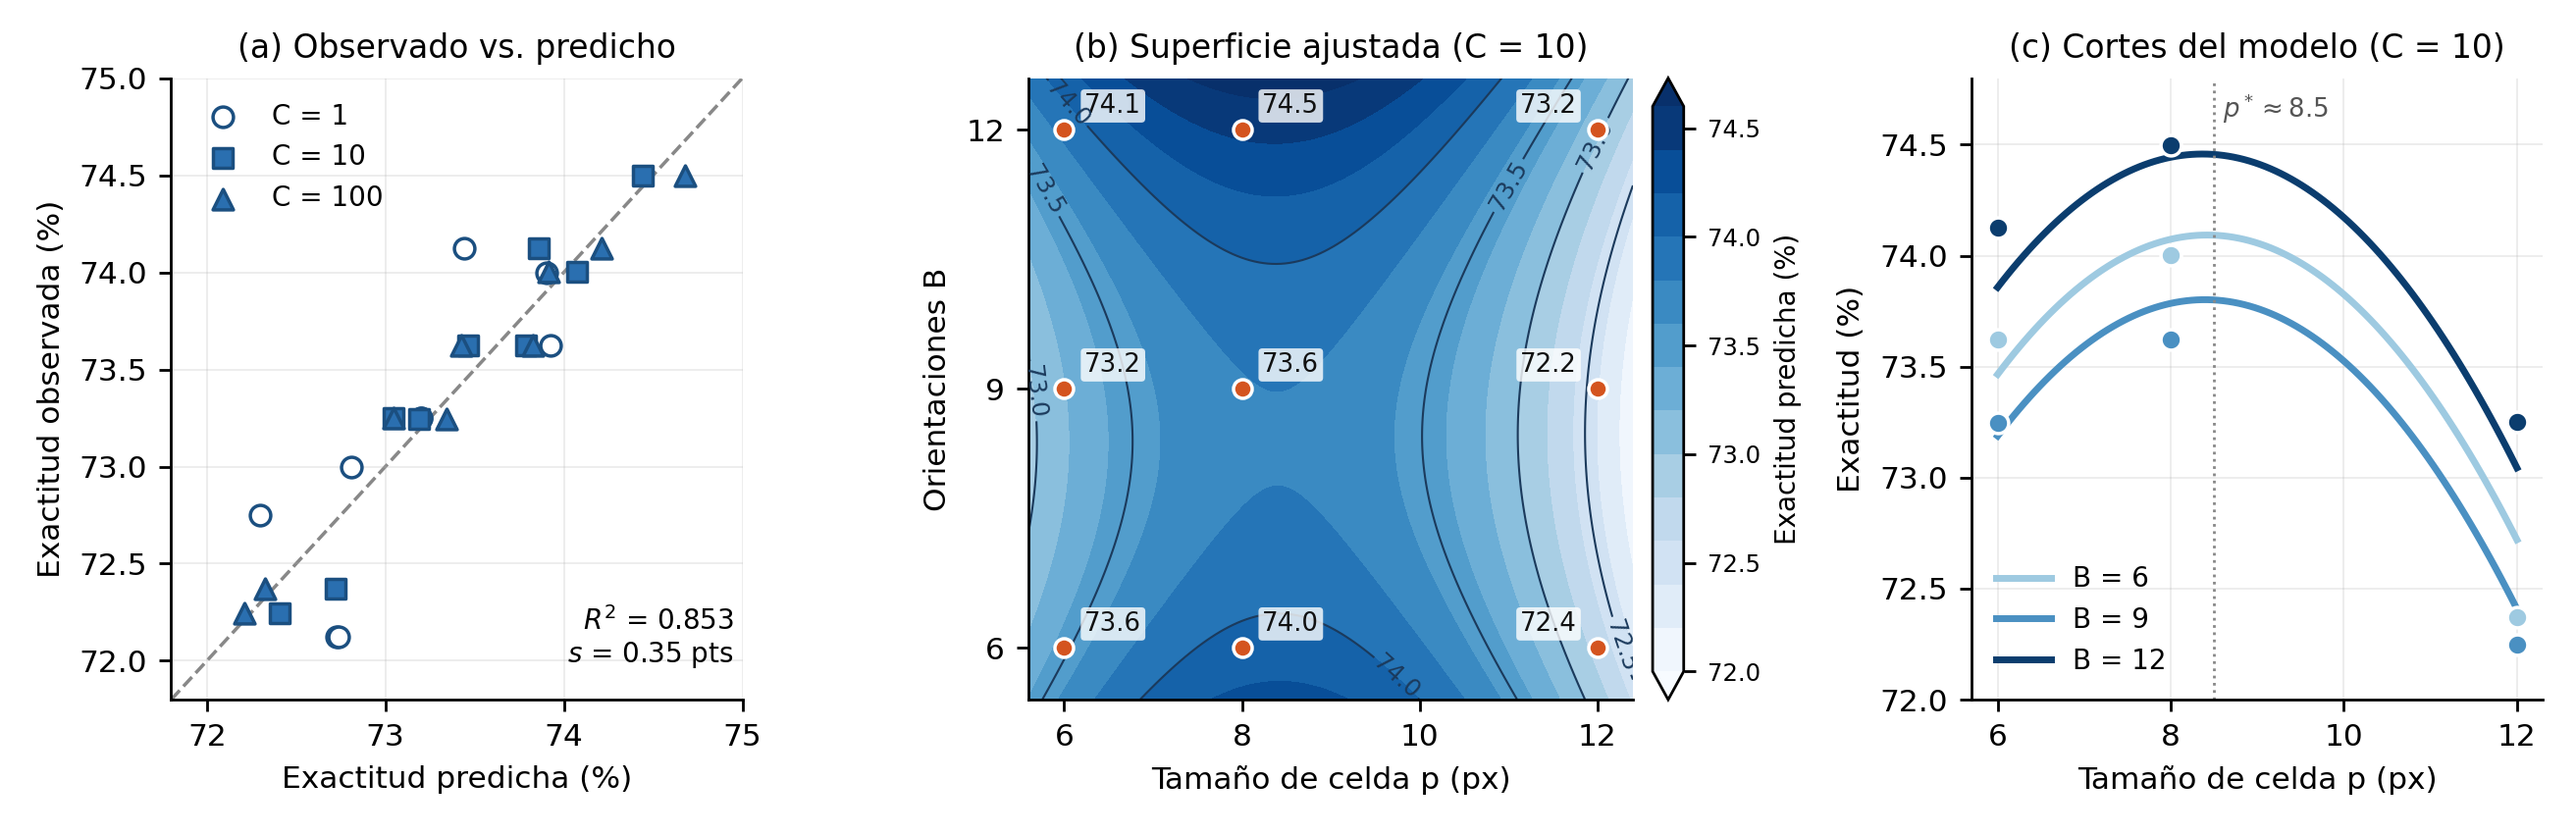
\includegraphics[width=\textwidth]{rsm_etapa1.png}
\caption{Reto 1: ajuste del modelo cuadrático (RSM) a las 27 corridas del factorial $3\times3\times3$. (a) Exactitud observada frente a la predicha por el modelo; la línea discontinua es la identidad y $s$ es la desviación estándar residual. (b) Superficie ajustada en el plano $p\times B$ para $C=10$; los puntos son las corridas y sus etiquetas la exactitud observada (\%). (c) Cortes del modelo a lo largo de $p$ para cada nivel de $B$ (líneas) junto con las observaciones (puntos); la línea punteada marca el óptimo $p^*\approx8.5$.}\label{fig:rsm1}
\end{figure*}

En el factorial $3\times3\times3$ sobre HOG y SVM, la mejor configuración fue $p=8$, $B=12$, $C=100$ (exactitud CV de 0.745). El modelo cuadrático explicó $R^2=0.853$ de la variación ($R^2_{\mathrm{aj}}=0.775$). Cuatro de sus nueve términos fueron significativos al 5\,\% (Tabla~\ref{tab:rsm1}): los términos lineal y cuadrático del tamaño de celda ($p<0.001$ en ambos) y los términos lineal y cuadrático del número de orientaciones ($p=0.007$ y $p=0.004$). Ninguno de los términos de $C$ fue significativo (lineal, $p=0.47$; cuadrático, $p=0.30$), y tampoco las interacciones: $p\times B$ ($p=0.87$) es despreciable, mientras que $p\times\log C$ ($p=0.09$) y $B\times\log C$ ($p=0.065$) quedaron cerca del umbral. En consecuencia, en la región explorada los efectos de $p$ y $B$ son aproximadamente separables y ambos son curvos, pero con curvatura de signo opuesto. En $p$, el término lineal positivo y el cuadrático negativo producen un máximo interior en $p^{*}\approx8.5$ píxeles (entre 8.1 y 8.7 según los valores de $B$ y $C$). En $B$, el término lineal negativo y el cuadrático positivo producen un mínimo cerca de $B\approx8$--$9$, de modo que la exactitud mejora hacia los extremos del rango explorado. En magnitud domina el tamaño de celda: a lo largo de su rango la exactitud predicha varía unos 1.4 puntos, frente a menos de 1 punto a lo largo de $B$; $C$ no influye. La Fig.~\ref{fig:rsm1} muestra la calidad del ajuste: las 27 corridas quedan alrededor de la identidad con una desviación residual de 0.35 puntos (Fig.~\ref{fig:rsm1}a), la superficie tiene forma de silla, con un máximo en $p\approx8.5$ a lo largo de $p$ y un mínimo en $B\approx8$--$9$ a lo largo de $B$ (Fig.~\ref{fig:rsm1}b), y los cortes del modelo siguen a las observaciones en los tres niveles de $B$ (Fig.~\ref{fig:rsm1}c). La falta de efecto de $C$ tiene una explicación directa: para $C=10$ y $C=100$ la exactitud es idéntica en las nueve combinaciones de $p$ y $B$, probablemente porque con 800 muestras en miles de dimensiones los datos de entrenamiento son separables y la SVM opera de hecho con margen duro, de modo que aumentar $C$ más allá de 10 no cambia la solución. En la práctica $C$ tuvo solo dos niveles efectivos, lo que también implica que los grados de libertad residuales del ajuste están algo sobreestimados.

\subsection{Análisis}
\textbf{Líneas base.} Reejecutadas con la misma partición, la imagen aplanada obtiene 0.605 en prueba (0.58 en clase) y HOG 0.685 en prueba frente a 0.734 en validación cruzada, lo que confirma que el 73\,\% reportado corresponde a validación cruzada y no a prueba. Con $D=67\,500\gg n=800$, las distancias euclídeas entre imágenes aplanadas quedan dominadas por brillo y posición; HOG reduce la dimensión a 8\,100 y codifica contornos con invariancia a iluminación (normalización por bloques) y a pequeñas traslaciones (histogramas por celda), lo que explica la ganancia de 8 puntos.

\textbf{Mejoras clásicas y su incertidumbre.} Los cuatro modelos N1, N2, N3 y N5 superan a la línea base HOG en prueba (0.705--0.720 frente a 0.685). Sin embargo, con 200 imágenes de prueba el error estándar de una exactitud cercana a 0.70 es $\sqrt{0.7\cdot0.3/200}\approx0.032$, es decir, un intervalo de confianza del 95\,\% de $\pm6$ puntos: las mejoras de 2 a 3.5 puntos son consistentes en dirección pero no concluyentes individualmente. El ensamble N5 no mejora sobre N3 porque sus componentes comparten el mismo descriptor y, por tanto, sus errores están fuertemente correlacionados ($\rho\to1$ anula el término $1/M$ de la varianza). El \emph{gradient boosting} (N4) ilustra el sobreajuste: 0.735 en validación cruzada pero 0.660 en prueba, esperable con 8\,772 características y 800 muestras.

\textbf{Mini-DoE.} El factorial reproduce en pequeño la tesis del proyecto doctoral: un barrido OFAT del número de orientaciones alrededor de la configuración de clase ($p=8$, $C=1$) habría encontrado diferencias menores de un punto, indistinguibles del ruido, y habría concluido que las orientaciones no importan. El diseño completo, en cambio, estima el efecto de $B$ combinando las 27 corridas, lo que reduce su incertidumbre y revela que es significativo y curvo, además de una interacción marginal con $C$. La diferencia entre la mejor configuración y la de clase (0.745 frente a 0.741) está, no obstante, dentro del ruido de la validación cruzada: una exactitud cercana a 0.74 estimada sobre 800 imágenes tiene una desviación estándar de $\sqrt{0.74\cdot0.26/800}\approx0.016$, es decir, unos 1.6 puntos, cuatro veces la diferencia observada (0.4 puntos). El diseño tampoco tiene réplicas, por lo que el error experimental se estima solo a partir de los residuos del modelo y no es posible una prueba de falta de ajuste. Para resolver diferencias de este tamaño sería necesario replicar cada corrida con varias particiones (validación cruzada repetida), lo que permite estimar el error puro, o aumentar el número de imágenes; incluir factores hoy fijos, como $\gamma$ o el tamaño de bloque, ampliaría además la región en la que la exactitud varía de forma apreciable.

\textbf{CNN desde cero.} La exactitud crece monotónicamente con la profundidad (0.580, 0.635 y 0.725 para 2, 3 y 4 bloques), coherente con el aumento del campo receptivo ($\sim2^L$), que permite pasar de bordes y texturas locales a partes del animal (orejas, hocico). Con 680 imágenes de entrenamiento, la CNN de 4 bloques apenas iguala al mejor modelo clásico. BatchNorm no aportó diferencia apreciable a profundidad 3 (0.635 frente a 0.625). Una primera ejecución con \emph{momentum} de BatchNorm de 0.99 y paciencia de 8 épocas produjo modelos que predecían una sola clase (exactitud de 0.50): con pocos pasos por época, las medias móviles usadas en inferencia no se estabilizan y el \emph{early stopping} restauró los pesos de la primera época; reducir el \emph{momentum} a 0.9 y retrasar el \emph{early stopping} resolvió el problema.

\textbf{Transferencia y autoencoder.} MobileNetV2 congelada alcanzó 0.945, 22.5 puntos por encima del mejor modelo clásico. La prueba de McNemar sobre las mismas 200 imágenes (51 aciertos solo de MobileNetV2 frente a 6 solo del ensamble) da $p=5.7\times10^{-10}$, por lo que la diferencia es significativa. Los filtros aprendidos en ImageNet ya separan categorías semánticas de animales, y solo se entrena la cabeza ($1280+1=1\,281$ parámetros). En contraste, el codificador del autoencoder (0.505) probablemente codifica sobre todo color y luminancia, información útil para minimizar $\|x-\hat x\|^2$ pero no discriminativa entre gatos y perros: la tarea de pretexto importa tanto como la arquitectura.

%----------------------------------------------------------------------
\section{Reto 2: 3Scenes}
\subsection{Datos y protocolo}
El conjunto 3scenes contiene tres clases de escena: costa, bosque y autopista (etiquetas originales \emph{coast}, \emph{forest} y \emph{highway}), en imágenes de $256\times256$. Las líneas base de clase son: momentos de color RGB ($\mu,\sigma$ por canal) con un perceptrón multicapa, partición 75/25 con \texttt{random\_state}=20 (exactitud 81\,\%, F1 macro 0.80), y una CNN secuencial Conv(8)-Conv(16)-Conv(32)+Dense entrenada 15 épocas, partición 75/25 con \texttt{random\_state}=40 (exactitud 88\,\%, F1 macro 0.87). En esta última, el conjunto de prueba se usa también como validación durante el entrenamiento. Aquí se adoptó una única partición de prueba (la de la CNN de clase, 240 imágenes), se separó un 15\,\% del entrenamiento como validación y la prueba solo se usó para la evaluación final; ambas líneas base se reejecutaron en estas condiciones.

\subsection{Modelos}
Además de replicar las líneas base (D0 es la CNN de clase con la misma arquitectura e hiperparámetros) se probaron dos versiones clásicas enriquecidas: momentos RGB y HSV más un histograma LBP de textura, con SVM (M1) y con MLP (M2). En aprendizaje profundo se entrenaron: una CNN de 4 bloques dobles con BatchNorm (\emph{momentum} 0.9), aumento de datos y \emph{global average pooling} (D1, 1.18\,M parámetros); MobileNetV2 congelada con entrada redimensionada a $224\times224$ (D2); la misma red con ajuste fino de las últimas 30 capas y $\eta=10^{-5}$ (D3); y un ensamble por promedio de probabilidades de D1 y D3 (D4).

\subsection{Resultados}
\begin{table*}[t]
\centering\caption{Reto 2: exactitud y F1 macro en prueba (240 imágenes).}\label{tab:r2}
\small
\renewcommand{\arraystretch}{1.15}\begin{tabular}{@{}llcr@{}}
\toprule
Familia & Modelo & Exactitud & F1 macro \\ \midrule
Clase (reportado) & RGB $\mu,\sigma$ + MLP & 0.812 & 0.80 \\
Clase (reportado) & CNN secuencial & 0.88 & 0.87 \\
Reejecutada & RGB $\mu,\sigma$ + MLP (partición rs=20) & 0.800 & 0.786 \\
Reejecutada & RGB $\mu,\sigma$ + MLP & 0.783 & 0.767 \\
\mk{r2s0}Reejecutada & CNN de clase (D0) & 0.917 & 0.915 \\
ML & RGB+HSV+LBP+SVM (M1) & 0.908 & 0.905\mk{r2e0} \\
ML & RGB+HSV+LBP+MLP (M2) & 0.888 & 0.884 \\
\mk{r2s1}DL & CNN+BN+aug.+GAP (D1) & 0.938 & 0.935 \\
DL & \textbf{MobileNetV2 congelada (D2)} & \textbf{0.983} & \textbf{0.983} \\
DL & \textbf{MobileNetV2 ajuste fino (D3)} & \textbf{0.983} & \textbf{0.983}\mk{r2e1} \\
DL & Ensamble D1+D3 (D4) & 0.983 & 0.983 \\ \bottomrule
\end{tabular}
%
\cajaf{r2s0}{r2e0}%
\cajaf{r2s1}{r2e1}%
\end{table*}

\begin{figure}[t]\centering
\fig{curvas_etapa2.png}{0.98\columnwidth}{curvas}
\caption{Curvas de entrenamiento: pérdida (izq.) y exactitud de validación (der.) de la CNN de clase (D0), la CNN propia (D1) y MobileNetV2 con ajuste fino (D3). En D0 la ``validación'' es el conjunto de prueba, como en el notebook de clase.}\label{fig:curvas2}
\end{figure}

\begin{figure}[t]\centering
\fig{cm_etapa2.png}{0.7\columnwidth}{cm2}
\caption{Matriz de confusión de MobileNetV2 con ajuste fino (D3) sobre las 240 imágenes de prueba de 3Scenes; entre paréntesis, el porcentaje de cada clase real.}\label{fig:cm2}
\end{figure}

\begin{table}[t]
\centering\caption{Reto 2: métricas por clase de MobileNetV2 con ajuste fino (D3) en prueba.}\label{tab:clases2}
\small
\begin{tabular}{@{}lcccc@{}}
\toprule
Clase & Precisión & Exhaustividad & F1 & Imágenes \\ \midrule
Costa & 0.966 & 0.988 & 0.977 & 85 \\
Bosque & 0.989 & 0.989 & 0.989 & 87 \\
Autopista & 1.000 & 0.971 & 0.985 & 68 \\ \midrule
Promedio macro & 0.985 & 0.982 & 0.983 & 240 \\
Promedio ponderado & 0.984 & 0.983 & 0.983 & 240 \\ \bottomrule
\end{tabular}
\end{table}

\begin{figure}[t]\centering
\fig{gradcam_etapa2.png}{0.98\columnwidth}{gc}
\caption{Grad-CAM de MobileNetV2: regiones que determinan la clase predicha. Los rótulos de la figura usan las etiquetas originales del conjunto (\emph{coast}: costa; \emph{forest}: bosque; \emph{highway}: autopista).}\label{fig:gc}
\end{figure}

\subsection{Relación entre textura y error}
Para cada imagen de prueba se calculó el número de esquinas FAST (y la varianza del Laplaciano) como \emph{proxy} de textura, y la tasa de error se estratificó por terciles para la línea base de color y para el mejor modelo (Tabla~\ref{tab:tex}). La textura visual condiciona la detección de \emph{features} y, con ello, la tasa de fallo de seguimiento en VI-SLAM.
\begin{table}[t]
\centering\caption{Tasa de error por tercil de textura (esquinas FAST), 80 imágenes por tercil.}\label{tab:tex}
\small
\begin{tabular}{@{}lcc@{}}
\toprule
Tercil de textura & RGB $\mu,\sigma$ + MLP & MobileNetV2 (D3) \\ \midrule
Baja & 0.263 (21) & 0.025 (2) \\
Media & 0.288 (23) & 0.013 (1) \\
Alta & 0.100 (8) & 0.013 (1) \\ \bottomrule
\end{tabular}
\end{table}

\subsection{Análisis}
\textbf{Línea base de color.} Reejecutada con su partición original, la línea base obtiene 0.800 (0.812 en clase; la diferencia probablemente se debe al orden de lectura de archivos y a la inicialización del MLP), y 0.783 en la partición común. Seis momentos de color separan bien bosque (verde, texturizado) de costa (azul), pero autopista comparte paleta con costa (cielo más superficie gris o azulada) y es la clase con menor F1 en clase (0.72). Añadir momentos HSV y un histograma LBP (M1) sube la exactitud a 0.908: la información de textura, por sí sola, lleva un modelo clásico por encima de la CNN reportada en clase (0.88).

\textbf{CNN de clase.} Reejecutada, D0 alcanzó 0.917, más que el 0.88 reportado; la diferencia refleja la variabilidad de una red sin semilla fija entrenada 15 épocas sin selección de modelo. Su pérdida de ``validación'' (que es la prueba) crece desde la época 5 mientras la de entrenamiento sigue bajando (Fig.~\ref{fig:curvas2}): la red sobreajusta. Tras tres \emph{poolings} el mapa es de $32\times32\times32$ y la capa densa concentra $32\,768\cdot3+3=98\,307$ de sus 104\,339 parámetros (94\,\%), una capa que memoriza posiciones en lugar de patrones. Además, usar la prueba como validación introduce un sesgo optimista en cualquier decisión tomada con esas curvas.

\textbf{CNN propia (D1).} Reemplazar \texttt{Flatten} por \emph{global average pooling}, duplicar la profundidad y añadir BatchNorm y aumento de datos lleva la exactitud a 0.938, con una pérdida de validación que se estabiliza en torno a 0.18 en lugar de crecer. Al igual que en el Reto 1, una primera ejecución con \emph{momentum} de BatchNorm de 0.99 y paciencia de 8 épocas falló (exactitud de 0.296, inferior al azar): el pico de pérdida de validación en la primera época (2.75 en la Fig.~\ref{fig:curvas2}) muestra la inestabilidad de las estadísticas de inferencia de BatchNorm con pocos pasos por época.

\textbf{Transferencia.} MobileNetV2 congelada ya alcanza 0.983 (4 errores en 240 imágenes: 2 de autopista, ambos clasificados como costa, 1 de costa y 1 de bosque; F1 por clase de 0.977, 0.989 y 0.985 para costa, bosque y autopista; Fig.~\ref{fig:cm2} y Tabla~\ref{tab:clases2}) con solo la cabeza entrenable ($1280\cdot3+3=3\,843$ parámetros). La matriz de confusión muestra que los únicos errores ocurren entre clases con componentes visuales compartidos: las dos imágenes de autopista mal clasificadas se asignaron a costa, que comparte con ella un cielo amplio y un horizonte despejado, mientras que bosque y autopista, visualmente muy distintas, nunca se confundieron entre sí. Por eso autopista alcanza precisión perfecta (1.000) pero la menor exhaustividad (0.971), y costa, que recibe esos dos errores, tiene la menor precisión (0.966). El ajuste fino con $\eta=10^{-5}$ no cambió ninguna predicción: la exactitud de validación era 1.0 desde el inicio y no quedaba gradiente útil que aprovechar. Por la misma razón, el ensamble D4 no mejora sobre D3. Frente a la CNN de clase (20 errores frente a 4), hay 19 imágenes que solo acierta D3 y 3 que solo acierta D0; la prueba de McNemar exacta da $p=8.6\times10^{-4}$, por lo que la mejora es estadísticamente significativa.

\textbf{Interpretabilidad.} Los mapas Grad-CAM \cite{selvaraju2017} (Fig.~\ref{fig:gc}) muestran que la red atiende a rasgos semánticos plausibles: el punto de fuga de la vía en autopista, el follaje en bosque y la superficie del agua junto a la línea de horizonte en costa, y no al cielo, que es la región compartida entre clases. No se observan atajos evidentes en las muestras inspeccionadas.

\textbf{Textura como factor.} El error de la línea base de color depende fuertemente de la textura: 26--29\,\% en los terciles bajo y medio frente a 10\,\% en el alto. MobileNetV2, en cambio, se mantiene entre 1 y 2.5\,\% en los tres terciles. El efecto de la textura depende, por tanto, del algoritmo: es una interacción algoritmo$\times$entorno, precisamente el tipo de efecto que un análisis OFAT no puede estimar y que motiva el uso de diseños factoriales en la evaluación de sistemas VI-SLAM. Con pocos errores en el mejor modelo, este resultado es descriptivo y debe confirmarse con más datos.

%----------------------------------------------------------------------
\section{Reto 3: Detección aérea con VisDrone}
\subsection{Conjunto de datos y aplicación}
VisDrone2019-DET \cite{du2018} contiene imágenes de dron de resolución variable (hasta $\approx2000\times1500$\,px) con diez clases y gran proporción de objetos pequeños: peatón (persona de pie o caminando), persona (en otra postura, por ejemplo sentada), bicicleta, automóvil, furgoneta, camión, triciclo, triciclo con toldo, bus y motocicleta (etiquetas originales \emph{pedestrian}, \emph{people}, \emph{bicycle}, \emph{car}, \emph{van}, \emph{truck}, \emph{tricycle}, \emph{awning-tricycle}, \emph{bus} y \emph{motor}). Es un escenario relevante para plataformas móviles con cámara, análogo al de un sistema VI-SLAM en un robot aéreo.

\subsection{Diseño experimental}
Se aplicó un factorial $2^2$ con los factores A: tamaño de modelo de Ultralytics YOLOv8 \cite{jocher2023} (YOLOv8n, 3.0\,M parámetros, frente a YOLOv8s, 11.1\,M) y B: resolución de entrada ($\text{imgsz}=512$ frente a 800), codificados en $\pm1$ y ejecutados en orden aleatorizado. Los cuatro modelos partieron de pesos preentrenados en COCO y se entrenaron 30 épocas sobre las 6\,471 imágenes de entrenamiento con idénticos hiperparámetros: lote de 64, optimizador AdamW seleccionado automáticamente por Ultralytics ($\eta=7.14\times10^{-4}$), precisión mixta, aumento por mosaico desactivado en las últimas 10 épocas, semilla 0 e imágenes precargadas en RAM. Se evaluó sobre las 548 imágenes de validación. Las respuestas fueron mAP@0.5 (mAP50), mAP@0.5:0.95, latencia de inferencia por imagen (ms), costo computacional (GFLOPs) y recall de objetos pequeños (área $<32^2$\,px, IoU$\ge0.5$ y clase correcta, sobre 300 imágenes de validación con 13\,252 objetos pequeños, 4\,884 medianos y 506 grandes).

\subsection{Resultados}
\begin{table*}[t]
\centering\caption{Reto 3: resultados por configuración (validación). $D_{\mathrm{lat}}$ y $D_{\mathrm{GF}}$: deseabilidad con costo en latencia o en GFLOPs, pesos $(2,1,1)$.}\label{tab:r3}
\small
\renewcommand{\arraystretch}{1.15}\begin{tabular}{@{}lccccccccr@{}}
\toprule
\multirow{2}{*}{Modelo} & \multirow{2}{*}{imgsz} & \multirow{2}{*}{mAP50} & \multirow{2}{*}{mAP50-95} & Recall obj. & Latencia & \multirow{2}{*}{GFLOPs} & Entrenamiento & \multirow{2}{*}{$D_{\mathrm{lat}}$} & \multirow{2}{*}{$D_{\mathrm{GF}}$} \\
 & & & & pequeños & (ms) & & (min) & & \\ \midrule
YOLOv8n & 512 & 0.229 & 0.125 & 0.225 & 0.19 & 5.2 & 3.0 & 0.49 & 0.49 \\
\mk{r3s0}YOLOv8n & 800 & 0.340 & 0.195 & 0.364 & 0.33 & 12.8 & 5.7 & 0.87 & \textbf{0.83}\mk{r3e0} \\
YOLOv8s & 512 & 0.306 & 0.173 & 0.307 & 0.33 & 18.3 & 4.1 & 0.76 & 0.70 \\
\mk{r3s1}YOLOv8s & 800 & \textbf{0.428} & \textbf{0.253} & \textbf{0.452} & 0.76 & 44.8 & 8.4 & \textbf{1.00} & 0.58\mk{r3e1} \\ \bottomrule
\end{tabular}
%
\cajaf{r3s0}{r3e0}%
\cajaf{r3s1}{r3e1}%
\end{table*}

\begin{table}[t]
\centering\caption{Reto 3: coeficientes del modelo $Y=\beta_0+\beta_Ax_A+\beta_Bx_B+\beta_{AB}x_Ax_B$ (factores codificados en $\pm1$; $\beta=E/2$) y contribución porcentual de cada término a la variación total ($SS_j/SS_T$, con $SS_j=E_j^2$ en un $2^2$ sin réplicas).}\label{tab:ef}
\footnotesize
\setlength{\tabcolsep}{3.5pt}
\renewcommand{\arraystretch}{1.15}\begin{tabular}{@{}lrrrrrrr@{}}
\toprule
Respuesta & $\beta_0$ & $\beta_A$ & $\beta_B$ & $\beta_{AB}$ & \%A & \%B & \%AB \\ \midrule
\mk{efs0}mAP50 & 0.326 & 0.041 & 0.058 & 0.003 & 33.5 & 66.4 & 0.1\mk{efe0} \\
mAP50-95 & 0.186 & 0.027 & 0.038 & 0.003 & 33.0 & 66.7 & 0.3 \\
Recall peq. & 0.337 & 0.043 & 0.071 & 0.002 & 26.5 & 73.5 & 0.0 \\
\mk{efs1}Latencia (ms) & 0.404 & 0.143 & 0.142 & 0.072 & 44.5 & 44.2 & 11.3 \\
GFLOPs & 20.30 & 11.27 & 8.50 & 4.72 & 57.3 & 32.6 & 10.1\mk{efe1} \\ \bottomrule
\end{tabular}
%
\cajaf{efs0}{efe0}%
\cajaf{efs1}{efe1}%
\end{table}

\begin{figure}[t]\centering
\fig{interaccion_etapa3.png}{0.98\columnwidth}{int}
\caption{Gráficas de interacción modelo$\times$resolución para mAP50, recall de objetos pequeños y latencia.}\label{fig:int}
\end{figure}

\begin{figure}[t]\centering
\fig{ap_por_clase_etapa3.png}{0.98\columnwidth}{ap}
\caption{AP50 por clase para las cuatro configuraciones.}\label{fig:ap}
\end{figure}

El recall por tamaño de objeto de la mejor configuración (YOLOv8s a 800) fue de 0.452 para objetos pequeños, 0.783 para medianos y 0.907 para grandes; en YOLOv8n a 512 los valores correspondientes fueron 0.225, 0.631 y 0.838. Por clase (Fig.~\ref{fig:ap}), la mejor configuración alcanzó un AP50 de 0.812 en automóvil, 0.574 en bus y 0.491 en peatón, y los valores más bajos en bicicleta (0.177) y triciclo con toldo (0.162). El entrenamiento de las cuatro corridas sumó 21.2 minutos de GPU (1\,272\,s).

\subsection{Trade-off mediante deseabilidad}
\begin{table}[t]
\centering\caption{Reto 3: deseabilidad compuesta $D_{\mathrm{GF}}$ (costo en GFLOPs) para distintos pesos $(w_{\mathrm{mAP}},w_{\mathrm{costo}},w_{\mathrm{rec}})$. En negrita, la mejor configuración de cada fila; el recuadro marca la columna que se discute en el texto.}\label{tab:des}
\small
\renewcommand{\arraystretch}{1.15}\begin{tabular}{@{}lrrrr@{}}
\toprule
Pesos & n-512 & n-800 & s-512 & s-800 \\ \midrule
$(1,1,1)$ & 0.567\mk{desa} & \textbf{0.856} & 0.722 & 0.488 \\
$(2,1,1)$ & 0.490 & \textbf{0.831} & 0.697 & 0.584 \\
$(1,2,1)$ & 0.653 & \textbf{0.849} & 0.718 & 0.340 \\
$(1,1,2)$ & 0.571 & \textbf{0.890} & 0.754 & 0.584 \\
$(1,3,1)$ & 0.710 & \textbf{0.844}\mk{desb} & 0.715 & 0.274 \\ \midrule
$D_{\mathrm{lat}}$, $(2,1,1)$ & 0.490 & 0.872 & 0.761 & \textbf{1.000} \\ \bottomrule
\end{tabular}
%
\begin{tikzpicture}[remember picture,overlay]\draw[caja] ([xshift=3pt]desat) rectangle ([xshift=3pt]desbb);\end{tikzpicture}%
\end{table}

Se combinaron mAP50 (maximizar, $L=0.15$, $T=0.40$), un costo computacional (minimizar) y el recall de objetos pequeños (maximizar, $L=0.05$, $T=0.35$) con $r=1$. Con el costo medido como latencia ($T=8$\,ms, $U=40$\,ms, pensados para una plataforma embebida), las cuatro configuraciones quedan por debajo de 1\,ms en la GPU de centro de datos, de modo que $d_{\mathrm{lat}}=1$ en todas y la deseabilidad se reduce a la precisión: gana YOLOv8s a 800 ($D=1.00$). Con el costo medido en GFLOPs, una medida independiente del \emph{hardware} ($T=5$, $U=50$), la configuración óptima pasa a ser YOLOv8n a 800 ($D=0.83$ frente a 0.58 de YOLOv8s a 800). Esta elección es robusta a los pesos (Tabla~\ref{tab:des}): YOLOv8n a 800 obtiene la mayor $D_{\mathrm{GF}}$ con los cinco juegos de pesos probados (0.83--0.89), mientras que la de YOLOv8s a 800 cae hasta 0.27 cuando se prioriza el costo. Los límites $L$, $T$ y $U$ son supuestos del autor y deben ajustarse a los requisitos de cada aplicación.

\subsection{Análisis}
\textbf{La resolución domina.} El efecto de la resolución sobre mAP50 ($E_B=0.116$, 66\,\% de la variación) supera al del tamaño de modelo ($E_A=0.083$, 34\,\%), y la diferencia es mayor en el recall de objetos pequeños ($0.142$ frente a $0.085$). La explicación es geométrica: un peatón de 20\,px en una imagen de 2\,000\,px de ancho queda en $20\cdot512/2000\approx5$\,px a $\text{imgsz}=512$, por debajo del \emph{stride} mínimo (8\,px) de la cabeza de detección de mayor resolución, mientras que a 800 ocupa $\approx8$\,px. En VisDrone el 71\,\% de los objetos evaluados son pequeños, por lo que aumentar la resolución recupera información que ninguna capacidad adicional del modelo puede reconstruir.

\textbf{Resolución frente a capacidad a igual costo.} YOLOv8n a 800 (12.8 GFLOPs) supera a YOLOv8s a 512 (18.3 GFLOPs) en mAP50 (0.340 frente a 0.306) y en recall de objetos pequeños (0.364 frente a 0.307) con un 30\,\% menos de cómputo. Para este dominio, invertir cómputo en resolución es más eficiente que invertirlo en capacidad.

\textbf{Interacción.} Sobre la precisión la interacción es prácticamente nula ($E_{AB}=0.005$ en mAP50, 0.1\,\% de la variación total; Tabla~\ref{tab:ef}): los efectos son aditivos y las rectas de la Fig.~\ref{fig:int} son casi paralelas. Sobre la latencia, en cambio, la interacción es del mismo orden que los efectos principales ($E_{AB}=0.144$\,ms): los GFLOPs crecen con el número de píxeles, $(800/512)^2\approx2.44$, y ese factor multiplica un costo base 3.5 veces mayor en YOLOv8s (18.3 frente a 5.2 GFLOPs a 512). Aumentar a la vez el modelo y la resolución es, por tanto, desproporcionadamente caro, un efecto que un análisis OFAT no habría revelado.

\textbf{Clases.} Las clases grandes y frecuentes (automóvil, bus) se detectan mejor; las pequeñas, finas o escasas (bicicleta, triciclo con toldo) son las peores. Los pares peatón/persona (0.491 frente a 0.363) y triciclo/triciclo con toldo (0.323 frente a 0.162) se distinguen por detalles de pocos píxeles (postura, toldo) y concentran confusiones.

\textbf{El \emph{hardware} como factor.} La configuración óptima cambia según cómo se mida el costo: con latencias de una GPU de centro de datos el \emph{trade-off} desaparece y gana el modelo más grande, mientras que con un costo representativo de una plataforma limitada gana el modelo pequeño a alta resolución. Este resultado respalda el planteamiento del proyecto doctoral de incluir las características del \emph{hardware} como factores explícitos del diseño experimental en lugar de fijarlas.

\subsection{Limitaciones}
Con una única réplica el diseño $2^2$ es saturado (4 corridas, 4 coeficientes) y los efectos son descriptivos, no inferenciales. Además, la precarga en RAM puede introducir pequeñas variaciones no deterministas, las latencias corresponden a inferencia por lotes en una GPU de centro de datos, y el recall por tamaño se calculó sobre 300 de las 548 imágenes de validación. La extensión natural es repetir con tres semillas para estimar error puro y realizar un ANOVA, añadir puntos centrales y axiales (CCD) para modelar curvatura, como se plantea en la Fase 2 del proyecto doctoral, y medir la latencia en el \emph{hardware} de destino.

%----------------------------------------------------------------------
\section{Discusión general y conexión con VI-SLAM}
Los tres retos comparten un patrón: la ganancia de rendimiento proviene de decisiones (descriptor, profundidad, resolución) que interactúan entre sí. El enfoque OFAT selecciona configuraciones subóptimas cuando existen interacciones; el diseño factorial permite estimarlas con pocas corridas. En VI-SLAM los factores análogos son el número de \emph{features}, la textura del entorno y la calidad del IMU, y las respuestas ATE \cite{sturm2012}, tasa de fallo de seguimiento y consumo computacional. Los ejercicios aquí presentados constituyen un ensayo del pipeline: diseño $\to$ ejecución aleatorizada $\to$ efectos $\to$ deseabilidad.

%----------------------------------------------------------------------
\section{Conclusiones}
En Cats\&Dogs, MobileNetV2 congelada alcanzó 94.5\,\% de exactitud en prueba frente a 68.5\,\% de la línea base HOG reejecutada y 72\,\% del mejor modelo clásico ($p=5.7\times10^{-10}$), mientras que las CNN entrenadas desde cero con 680 imágenes no superaron el 72.5\,\%. En 3Scenes, MobileNetV2 alcanzó 98.3\,\% frente a 88\,\% reportado y 91.7\,\% reejecutado para la CNN de clase ($p=8.6\times10^{-4}$), y un modelo clásico con textura (90.8\,\%) también superó la línea base convolucional. El error del clasificador de color dependió de la textura de la escena y el del modelo profundo no, una interacción algoritmo$\times$entorno. En VisDrone, la resolución de entrada fue el factor dominante de la precisión y la configuración óptima dependió de cómo se mide el costo computacional: YOLOv8s a 800 si solo importa la precisión, YOLOv8n a 800 si se penaliza el cómputo. Como trabajo futuro se plantea replicar los diseños con varias semillas, extenderlos a diseños de superficie de respuesta y trasladar el mismo protocolo a la evaluación de sistemas VI-SLAM en simulación y en \emph{hardware} real.

\section*{Reproducibilidad}
Se usaron semillas fijas, particiones fijas y cuadernos ejecutables (\texttt{Etapa1\_CatsDogs}, \texttt{Etapa2\_3Scenes} y \texttt{Etapa3\_VisDrone\_DoE}). Los cuadernos, los archivos de resultados (CSV), las figuras y los pesos entrenados están disponibles en \url{https://github.com/miltoneufrasio/evaluacion_vision_slam/tree/main/ejercicio-2}.

\section*{Declaración de uso de inteligencia artificial}
En la elaboración de este trabajo se utilizó un asistente de inteligencia artificial generativa (Claude, Anthropic) como apoyo en la redacción y revisión del texto y en la depuración y corrección de los códigos. El diseño de los experimentos, su ejecución, la verificación de los resultados y las conclusiones son responsabilidad del autor, quien revisó y validó todo el contenido.

\begin{thebibliography}{99}
% Referencias en formato APA 7 (orden alfabético); DOI y URL como hiperenlaces
\bibitem{dalal2005} Dalal, N., \& Triggs, B. (2005). Histograms of oriented gradients for human detection. En \emph{2005 IEEE Computer Society Conference on Computer Vision and Pattern Recognition (CVPR'05)} (Vol.~1, pp.~886--893). IEEE. \url{https://doi.org/10.1109/CVPR.2005.177}
\bibitem{derringer1980} Derringer, G., \& Suich, R. (1980). Simultaneous optimization of several response variables. \emph{Journal of Quality Technology, 12}(4), 214--219. \url{https://doi.org/10.1080/00224065.1980.11980968}
\bibitem{jocher2023} Jocher, G., Chaurasia, A., \& Qiu, J. (2023). \emph{Ultralytics YOLOv8} (Versión 8.0.0) [Software]. \url{https://github.com/ultralytics/ultralytics}
\bibitem{googleg4} Kim, R., \& Vu, D. (2025, 20 de octubre). G4 VMs powered by NVIDIA RTX PRO 6000 Blackwell GPUs are GA. \emph{Google Cloud Blog}. \url{https://cloud.google.com/blog/products/compute/g4-vms-powered-by-nvidia-rtx-6000-blackwell-gpus-are-ga}
\bibitem{kingma2015} Kingma, D.~P., \& Ba, J. (2015). Adam: A method for stochastic optimization. En \emph{3rd International Conference on Learning Representations (ICLR 2015)}. \url{https://doi.org/10.48550/arXiv.1412.6980}
\bibitem{loshchilov2019} Loshchilov, I., \& Hutter, F. (2019). Decoupled weight decay regularization. En \emph{7th International Conference on Learning Representations (ICLR 2019)}. \url{https://doi.org/10.48550/arXiv.1711.05101}
\bibitem{mcnemar1947} McNemar, Q. (1947). Note on the sampling error of the difference between correlated proportions or percentages. \emph{Psychometrika, 12}(2), 153--157. \url{https://doi.org/10.1007/BF02295996}
\bibitem{montgomery2019} Montgomery, D.~C. (2019). \emph{Design and analysis of experiments} (10.\textsuperscript{a} ed.). Wiley.
\bibitem{myers2016} Myers, R.~H., Montgomery, D.~C., \& Anderson-Cook, C.~M. (2016). \emph{Response surface methodology: Process and product optimization using designed experiments} (4.\textsuperscript{a} ed.). Wiley.
\bibitem{ojala2002} Ojala, T., Pietikäinen, M., \& Mäenpää, T. (2002). Multiresolution gray-scale and rotation invariant texture classification with local binary patterns. \emph{IEEE Transactions on Pattern Analysis and Machine Intelligence, 24}(7), 971--987. \url{https://doi.org/10.1109/TPAMI.2002.1017623}
\bibitem{sandler2018} Sandler, M., Howard, A., Zhu, M., Zhmoginov, A., \& Chen, L.-C. (2018). MobileNetV2: Inverted residuals and linear bottlenecks. En \emph{2018 IEEE/CVF Conference on Computer Vision and Pattern Recognition} (pp.~4510--4520). IEEE. \url{https://doi.org/10.1109/CVPR.2018.00474}
\bibitem{selvaraju2017} Selvaraju, R.~R., Cogswell, M., Das, A., Vedantam, R., Parikh, D., \& Batra, D. (2017). Grad-CAM: Visual explanations from deep networks via gradient-based localization. En \emph{2017 IEEE International Conference on Computer Vision (ICCV)} (pp.~618--626). IEEE. \url{https://doi.org/10.1109/ICCV.2017.74}
\bibitem{sturm2012} Sturm, J., Engelhard, N., Endres, F., Burgard, W., \& Cremers, D. (2012). A benchmark for the evaluation of RGB-D SLAM systems. En \emph{2012 IEEE/RSJ International Conference on Intelligent Robots and Systems} (pp.~573--580). IEEE. \url{https://doi.org/10.1109/IROS.2012.6385773}
\bibitem{du2018} Zhu, P., Wen, L., Du, D., Bian, X., Ling, H., Hu, Q., et al. (2019). VisDrone-DET2018: The vision meets drone object detection in image challenge results. En L. Leal-Taixé \& S. Roth (Eds.), \emph{Computer Vision -- ECCV 2018 Workshops} (Lecture Notes in Computer Science, Vol.~11133). Springer, Cham. \url{https://doi.org/10.1007/978-3-030-11021-5_27}
\end{thebibliography}

\end{document}
